\documentclass{beamer}

\usetheme{Boadilla}

\title[edytory]{Linux}
\subtitle{Edytory tekstu}

\author{Alan Guła}
\date{\today}

\begin{document}

\begin{frame}
    \titlepage
\end{frame}

\begin{frame}{Spis treści}
    \tableofcontents
\end{frame}

\section{Wprowadzenie}
\begin{frame}{Wprowadzenie}
Edytory tekstu w systemie Linux sa niezbednym narzedziem do pracy z plikami tekstowymi, 
kodem zrodlowym czy konfiguracjami systemowymi. Dwa popularne edytory, ktore oferuje Linux, 
to Vim i Nano. Oba posiadaja swoje unikalne cechy, a ich wybor zalezy od preferencji uzytkownika oraz stopnia zaawansowania.
Dokument ten przedstawi podstawowa obsluge edytorow vim oraz nano.
\end{frame}

\subsection{Vim}
\begin{frame}{Vim}
Vim to zaawansowany edytor tekstu, ktory jest rozwinieciem klasycznego edytora Vi. Jest bardzo popularny wsrod programistow i administratorow systemow ze wzgledu na swoje zaawansowane funkcje i mozliwosci. Vim oferuje tryby pracy: normalny, wstawiania i komend. Jego zaleta jest szybkosć i efektywnosć w obsludze duzych plikow oraz wsparcie dla wielu jezykow programowania. Jednak, dla nowych uzytkownikow moze być trudny w nauce, poniewaz wiekszosć operacji odbywa sie za pomoca skrotow klawiszowych i komend.
\end{frame}

\subsection{Nano}
\begin{frame}{Nano}
Nano to prostszy edytor tekstu, ktory oferuje intuicyjny interfejs. Jest bardziej przystepny dla poczatkujacych uzytkownikow, poniewaz nie wymaga znajomosci trybow czy skomplikowanych komend. Wystarczy uruchomić go, zaczać pisać, a na dole ekranu znajduja sie informacje o dostepnych skrotach klawiszowych, co ulatwia korzystanie z edytora. Nano jest idealnym wyborem dla osob, ktore potrzebuja prostego narzedzia do szybkiej edycji plikow tekstowych bez potrzeby zaawansowanej konfiguracji.
\end{frame}

\section{Vim}
\begin{frame}{Vim}
\centering

\includegraphics{vim.png}
\end{frame}

\subsection{Co to jest Vim?}
\begin{frame}{Co to jest Vim?}
Vim to zaawansowany edytor tekstu, ktory jest czesto uzywany w systemach Linux.
\end{frame}

\subsection{Uruchamianie Vim}
\begin{frame}{Uruchamianie Vim}
Aby otworzyc plik w Vim, uzyj polecenia:
vim nazwapliku.txt
\end{frame}

\subsection{Podstawowe tryby}
\begin{frame}{Podstawowe tryby}
\begin{itemize}
\item Tryb normalny - Domyslny tryb w ktorym mozna poruszac sie po pliku i wydawac polecenia
\item Tryb edycji - Tryb w ktorym mozna edytowac tekst. Uruchamia sie po kliknieciu i lub a w trybie normalnym. Mozna z niego wyjsc klikajac *Esc*.
\end{itemize}
\end{frame}

\subsection{Podsumowanie}
\begin{frame}{Podsumowanie}
Vim z poczatku moze sie wydawac trudny, ale po nabyciu wprawy okazuje sie, ze jest poteznym narzedziem.
\end{frame}

\section{Nano}
\begin{frame}{Nano}
\centering
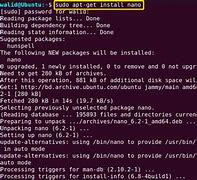
\includegraphics{nano.png}
\end{frame}

\subsection{Co to jest Nano?}
\begin{frame}{Co to jest Nano?}
Nano to prosty edytor tekstu dzialajacy w terminalu, popularny w systemach Linux.
\end{frame}

\subsection{Uruchamianie Nano}
\begin{frame}{Uruchamianie Nano}
Aby otworzyc plik w nano, uzyj polecenia:
nano nazwapliku.txt.
Po otwarciu juz mozna edytowac tekst.
\end{frame}

\subsection{Podstawowe skroty klawiszowe}
\begin{frame}{Podstawowe skroty klawiszowe}
\begin{itemize}
\item Ctrl + O   — zapisz plik.
\item Ctrl + X   — wyjdz z edytora. 
\item Ctrl + W   — wyszukaj tekst.
\item Ctrl + K   — wytnij tekst.
\item Ctrl + U   — wklej tekst.
\item Ctrl + C   — pokaz aktualna pozycje kursora.
\end{itemize}
\end{frame}

\subsection{Podsumowanie}
\begin{frame}{Podsumowanie}
Nano jest prostym, ale funkcjonalnym edytorem tekstu, idealnym dla poczatkujacych uzytkownikow.
\end{frame}


\section{Koniec}
\begin{frame}
\centering
Koniec
\end{frame}






\end{document}
